\documentclass{article}
\usepackage[utf8]{inputenc}

\usepackage{multirow}
\usepackage{multicol}
\usepackage{array}
\usepackage{graphicx}

\usepackage{tikz}

\usetikzlibrary{decorations.pathreplacing}
\usetikzlibrary{shapes.misc}
\definecolor{RoyalBlue}{RGB}{65, 105, 225}

\usetikzlibrary{quantikz}

\usepackage[landscape, paperwidth=15cm, paperheight=30cm, margin=0mm]{geometry}

\title{\vspace{-5ex}}
\date{\vspace{-5ex}}

\begin{document}

\scalebox{0.7}{
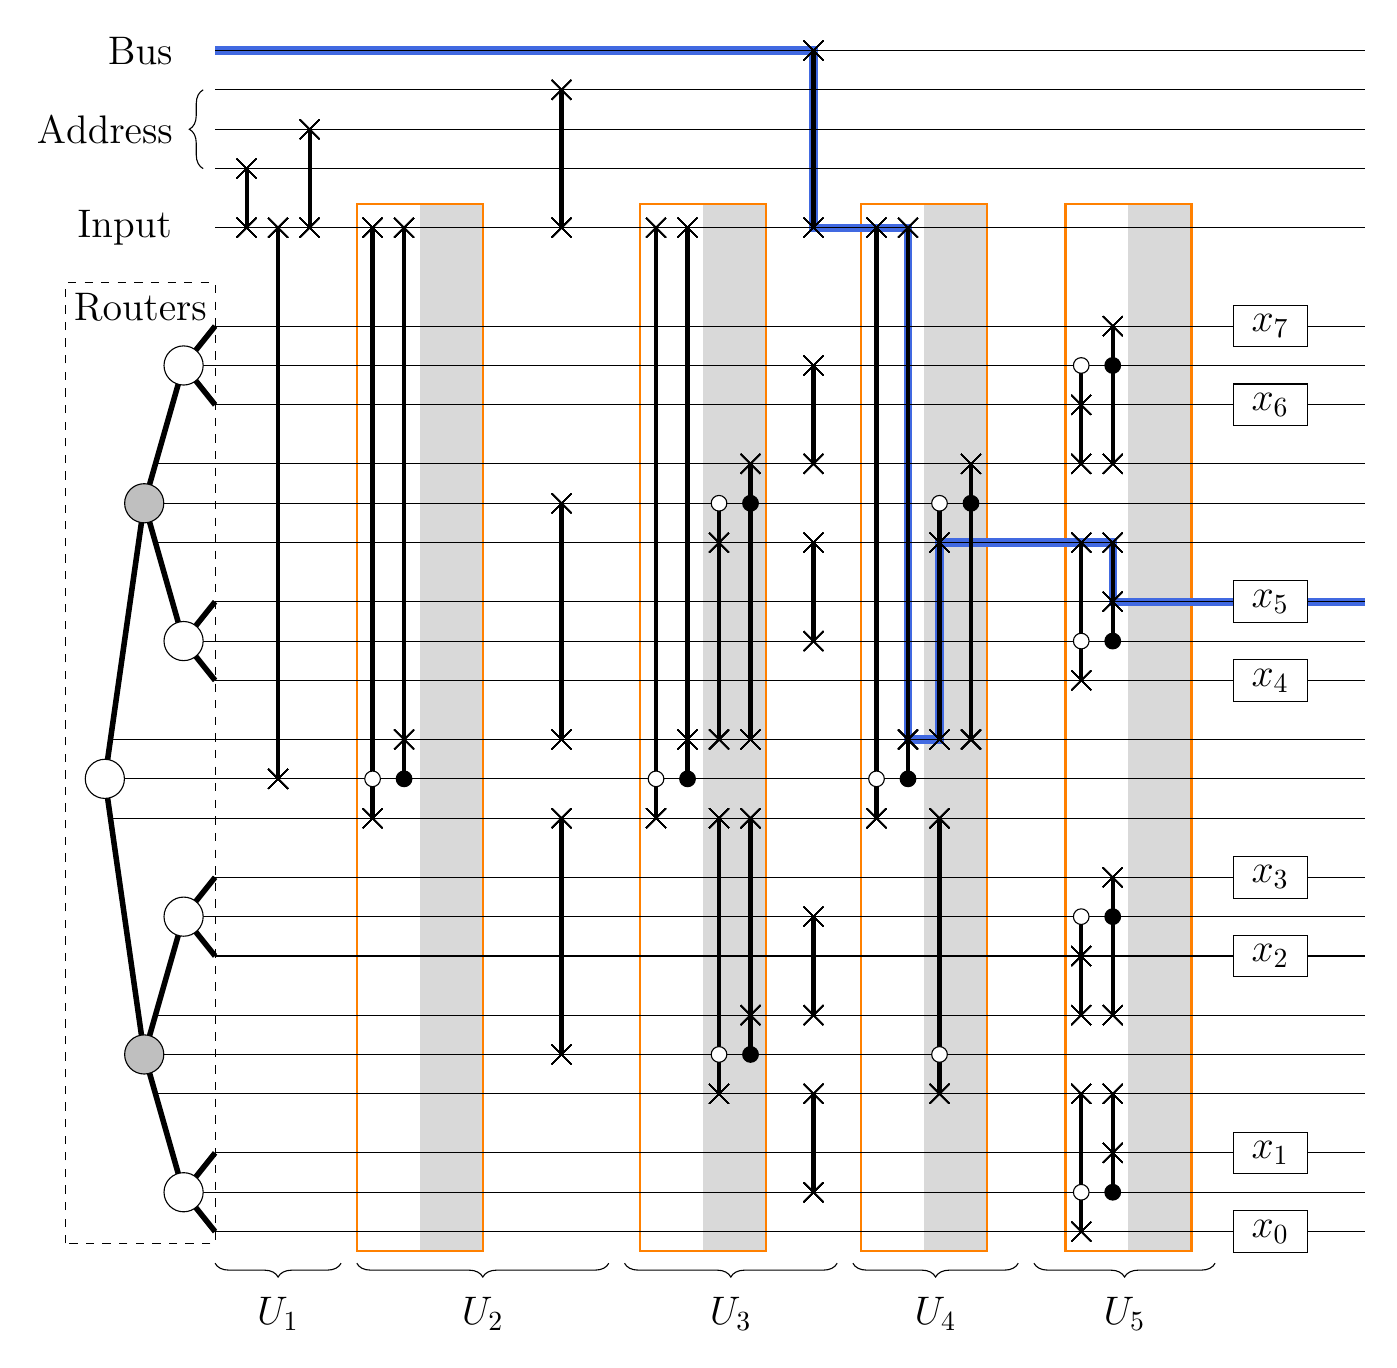
\begin{tikzpicture}
    % Define drawing element styles
    \tikzstyle{conn}=[-]
    \tikzstyle{connThick}=[-, line width = 2]
    \tikzstyle{whiteCirc}=[circle, draw, fill = white, inner sep = 5]
    \tikzstyle{grayCirc}=[circle, draw, fill = gray!50, inner sep = 5]
    \tikzstyle{every node}=[font=\Large]
    \tikzstyle{swap}=[-, line width = 2, mark = x, mark size = 5pt]
    \tikzstyle{connSwap}=[-, line width = 1.5]
    \tikzstyle{wc}=[circle, draw, fill=white, inner sep = 2]
    \tikzstyle{bc}=[circle, draw, fill=black, inner sep = 2]
    \tikzstyle{orangeRec}=[orange, thick]
    \tikzstyle{grayRec}=[gray!30]
    \tikzstyle{op}=[draw, fill = white, text width = 2em, align = center]
    \tikzstyle{blueLine}=[-, line width = 3, RoyalBlue]

    % Define variables 
    \def\xend{16.0} % The end of x-coordinate

    % Thick lines that connect the nodes
    \draw[connThick] (0,0) -- (0.5,3.5) ;
    \draw[connThick] (0,0) -- (0.5,-3.5) ;
    \draw[connThick] (0.5,3.5) -- (1.0, 5.25) ;
    \draw[connThick] (0.5,3.5) -- (1.0, 1.75) ;
    \draw[connThick] (0.5,-3.5) -- (1.0, -5.25) ;
    \draw[connThick] (0.5,-3.5) -- (1.0, -1.75) ;
    \draw[connThick] (1.0,1.75) -- (1.4, 2.25) ;
    \draw[connThick] (1.0,1.75) -- (1.4, 1.25) ;
    \draw[connThick] (1.0,5.25) -- (1.4, 5.75) ;
    \draw[connThick] (1.0,5.25) -- (1.4, 4.75) ;
    \draw[connThick] (1.0,-1.75) -- (1.4, -2.25) ;
    \draw[connThick] (1.0,-1.75) -- (1.4, -1.25) ;
    \draw[connThick] (1.0,-5.25) -- (1.4, -5.75) ;
    \draw[connThick] (1.0,-5.25) -- (1.4, -4.75) ;

    % Orange Rectangle 1
    \fill[grayRec] (4.0, -6.0) rectangle (4.8, 7.3);
    \draw[orangeRec] (3.2, -6.0) rectangle (4.8, 7.3);
    
    % Orange Rectangle 2
    \fill[grayRec] (7.6, -6.0) rectangle (8.4, 7.3);
    \draw[orangeRec] (6.8, -6.0) rectangle (8.4, 7.3);
    
    % Orange Rectangle 3
    \fill[grayRec] (10.4, -6.0) rectangle (11.2, 7.3);
    \draw[orangeRec] (9.6, -6.0) rectangle (11.2, 7.3);
    
    % Orange Rectangle 4
    \fill[grayRec] (13.0, -6.0) rectangle (13.8, 7.3);
    \draw[orangeRec] (12.2, -6.0) rectangle (13.8, 7.3);
    
    % Blue Line
    \draw[blueLine] (1.4, 9.25) -- (9.0, 9.25) -- (9.0, 7.0) -- (10.2, 7.0) -- (10.2, 0.5) -- (10.6, 0.5) -- (10.6, 3.0) -- (12.8, 3.0) -- (12.8, 2.25) -- (\xend, 2.25);
    
    
    % White node at the centre
    \draw[conn] (0.05, -0.5) -- (\xend, -0.5);
    \draw[conn] (0., 0) -- (\xend, 0);
    \draw[conn] (0.05, 0.5) -- (\xend, 0.5);
    \node[whiteCirc] at (0,0) {};

    % Gray nodes upper
    \draw[conn] (0.63, 3.0) -- (\xend, 3.0);
    \draw[conn] (0.5, 3.5) -- (\xend, 3.5);
    \draw[conn] (0.63, 4.0) -- (\xend, 4.0);
    \node[grayCirc] at (0.5,3.5) {};

    % Gray nodes lower
    \draw[conn] (0.63, -3.0) -- (\xend, -3.0);
    \draw[conn] (0.5, -3.5) -- (\xend, -3.5);
    \draw[conn] (0.63, -4.0) -- (\xend, -4.0);
    \node[grayCirc] at (0.5,-3.5) {};
    
    % white nodes upper upper
    \draw[conn] (1.4, 5.75) -- (\xend, 5.75);
    \draw[conn] (1.0, 5.25) -- (\xend, 5.25);
    \draw[conn] (1.4, 4.75) -- (\xend, 4.75);
    \node[whiteCirc] at (1.0,5.25) {};

    % white nodes upper lower
    \draw[conn] (1.4, 1.25) -- (\xend, 1.25);
    \draw[conn] (1.0, 1.75) -- (\xend, 1.75);
    \draw[conn] (1.4, 2.25) -- (\xend, 2.25);
    \node[whiteCirc] at (1.0,1.75) {};
    
    % white nodes lower lower
    \draw[conn] (1.4, -5.75) -- (\xend, -5.75);
    \draw[conn] (1.0, -5.25) -- (\xend, -5.25);
    \draw[conn] (1.4, -4.75) -- (\xend, -4.75);
    \node[whiteCirc] at (1.0,-5.25) {};

    % white nodes lower upper
    \draw[conn] (1.4, -1.25) -- (\xend, -1.25);
    \draw[conn] (1.0, -1.75) -- (\xend, -1.75);
    \draw[conn] (1.4, -2.25) -- (\xend, -2.25);
    \node[whiteCirc] at (1.0,-1.75) {};

    % Router rectangle
    \node at (0.45, 6.0) {Routers};
    \draw[dashed] (-0.5, -5.9) rectangle (1.4, 6.3); 

    % Input 
    \draw[conn] (1.4, 7.0) -- (\xend, 7.0);
    \node at (0.25, 7.0) {Input};

    % Address
    \draw[conn] (1.4, 7.75) -- (\xend, 7.75);
    \draw[conn] (1.4, 8.25) -- (\xend, 8.25);
    \draw[conn] (1.4, 8.75) -- (\xend, 8.75);
    \draw[decorate, decoration = {brace, amplitude = 5pt, raise = 1ex}] (1.4, 7.75) -- (1.4, 8.75);
    \node at (0.0, 8.25) {Address};

    % Bus
    \draw[conn] (1.4, 9.25) -- (\xend, 9.25);
    \node at (0.45, 9.25) {Bus};

    % Column 1
    \draw[connSwap] (1.8, 7.0) -- (1.8, 7.75);
    \draw plot[swap] (1.8, 7.0);
    \draw plot[swap] (1.8, 7.75);

    % Column 2 
    \draw[connSwap] (2.2, 7.0) -- (2.2, 0.0);
    \draw plot[swap] (2.2, 7.0);
    \draw plot[swap] (2.2, 0.0);
    
    % Column 3
    \draw[connSwap] (2.6, 7.0) -- (2.6, 8.25);
    \draw plot[swap] (2.6, 7.0);
    \draw plot[swap] (2.6, 8.25);

    % Column 4
    \draw[connSwap] (3.4, 7.0) -- (3.4, -0.5);
    \draw plot[swap] (3.4, 7.0);
    \draw plot[swap] (3.4, -0.5);
    \node[wc] at (3.4, 0.0) {};

    % Column 5
    \draw[connSwap] (3.8, 7.0) -- (3.8, 0.0);
    \draw plot[swap] (3.8, 7.0);
    \draw plot[swap] (3.8, 0.5);
    \node[bc] at (3.8, 0.0) {};

    % Column 6
    \draw[connSwap] (5.8, 7.0) -- (5.8, 8.75);
    \draw plot[swap] (5.8, 8.75);
    \draw plot[swap] (5.8, 7.0);
    
    \draw[connSwap] (5.8, 3.5) -- (5.8, 0.5);
    \draw plot[swap] (5.8, 3.5);
    \draw plot[swap] (5.8, 0.5);

    \draw[connSwap] (5.8, -0.5) -- (5.8, -3.5);
    \draw plot[swap] (5.8, -3.5);
    \draw plot[swap] (5.8, -0.5);

    % Column 7
    \draw[connSwap] (7.0, 7.0) -- (7.0, -0.5);
    \draw plot[swap] (7.0, 7.0);
    \draw plot[swap] (7.0, -0.5);
    \node[wc] at (7.0, 0.0) {};

    % Column 8 
    \draw[connSwap] (7.4, 7.0) -- (7.4, 0.0);
    \draw plot[swap] (7.4, 7.0);
    \draw plot[swap] (7.4, 0.5);
    \node[bc] at (7.4, 0.0) {};

    % Column 9
    \draw[connSwap] (7.8, 3.5) -- (7.8, 0.5);
    \draw plot[swap] (7.8, 3.0);
    \draw plot[swap] (7.8, 0.5);
    \node[wc] at (7.8, 3.5) {};
    
    \draw[connSwap] (7.8, -0.5) -- (7.8, -4.0);
    \draw plot[swap] (7.8, -4.0);
    \draw plot[swap] (7.8, -0.5);
    \node[wc] at (7.8, -3.5) {};

    % Column 10
    \draw[connSwap] (8.2, 0.5) -- (8.2, 4.0);
    \draw plot[swap] (8.2, 0.5);
    \draw plot[swap] (8.2, 4.0);
    \node[bc] at (8.2, 3.5) {};

    \draw[connSwap] (8.2, -0.5) -- (8.2, -3.5);
    \draw plot[swap] (8.2, -0.5);
    \draw plot[swap] (8.2, -3.0);
    \node[bc] at (8.2, -3.5) {};

    % Column 11
    \draw[connSwap] (9.0, 7.0) -- (9.0, 9.25);
    \draw plot[swap] (9.0, 7.0);
    \draw plot[swap] (9.0, 9.25);

    \draw[connSwap] (9.0, 5.25) -- (9.0, 4.0);
    \draw plot[swap] (9.0, 5.25);
    \draw plot[swap] (9.0, 4.0);

    \draw[connSwap] (9.0, 3.0) -- (9.0, 1.75);
    \draw plot[swap] (9.0, 1.75);
    \draw plot[swap] (9.0, 3.0);
    
    \draw[connSwap] (9.0, -5.25) -- (9.0, -4.0);
    \draw plot[swap] (9.0, -5.25);
    \draw plot[swap] (9.0, -4.0);

    \draw[connSwap] (9.0, -3.0) -- (9.0, -1.75);
    \draw plot[swap] (9.0, -1.75);
    \draw plot[swap] (9.0, -3.0);

    % Column 12
    \draw[connSwap] (9.8, 7.0) -- (9.8, -0.5);
    \draw plot[swap] (9.8, 7.0);
    \draw plot[swap] (9.8, -0.5);
    \node[wc] at (9.8, 0.0) {};

    % Column 13
    \draw[connSwap] (10.2, 7.0) -- (10.2, 0.0);
    \draw plot[swap] (10.2, 7.0);
    \draw plot[swap] (10.2, 0.5);
    \node[bc] at (10.2, 0.0) {};

    % Column 14
    \draw[connSwap] (10.6, 3.5) -- (10.6, 0.5);
    \draw plot[swap] (10.6, 3.0);
    \draw plot[swap] (10.6, 0.5);
    \node[wc] at (10.6, 3.5) {};
    
    \draw[connSwap] (10.6, -0.5) -- (10.6, -4.0);
    \draw plot[swap] (10.6, -4.0);
    \draw plot[swap] (10.6, -0.5);
    \node[wc] at (10.6, -3.5) {};

    % Column 15
    \draw[connSwap] (11.0, 0.5) -- (11.0, 4.0);
    \draw plot[swap] (11.0, 0.5);
    \draw plot[swap] (11.0, 4.0);
    \node[bc] at (11.0, 3.5) {};

    % Column 16
    \draw[connSwap] (12.4, 4.0) -- (12.4, 5.25);
    \draw plot[swap] (12.4, 4.0);
    \draw plot[swap] (12.4, 4.75);
    \node[wc] at (12.4, 5.25) {};

    \draw[connSwap] (12.4, 3.0) -- (12.4, 1.25);
    \draw plot[swap] (12.4, 3.0);
    \draw plot[swap] (12.4, 1.25);
    \node[wc] at (12.4, 1.75) {};

    \draw[connSwap] (12.4, -1.75) -- (12.4, -3.0);
    \draw plot[swap] (12.4, -2.25);
    \draw plot[swap] (12.4, -3.0);
    \node[wc] at (12.4, -1.75) {};

    \draw[connSwap] (12.4, -4.0) -- (12.4, -5.75);
    \draw plot[swap] (12.4, -4.0);
    \draw plot[swap] (12.4, -5.75);
    \node[wc] at (12.4, -5.25) {};

    % Column 17
    \draw[connSwap] (12.8, 5.75) -- (12.8, 4.0);
    \draw plot[swap] (12.8, 5.75);
    \draw plot[swap] (12.8, 4.0);
    \node[bc] at (12.8, 5.25) {};

    \draw[connSwap] (12.8, 3.0) -- (12.8, 1.75);
    \draw plot[swap] (12.8, 3.0);
    \draw plot[swap] (12.8, 2.25);
    \node[bc] at (12.8, 1.75) {};

    \draw[connSwap] (12.8, -1.25) -- (12.8, -3.0);
    \draw plot[swap] (12.8, -1.25);
    \draw plot[swap] (12.8, -3.0);
    \node[bc] at (12.8, -1.75) {};

    \draw[connSwap] (12.8, -4.0) -- (12.8, -5.25);
    \draw plot[swap] (12.8, -4.0);
    \draw plot[swap] (12.8, -4.75);
    \node[bc] at (12.8, -5.25) {};

    % Text Column
    \node[op] at (14.8, 5.75) {$x_7$};
    \node[op] at (14.8, 4.75) {$x_6$};
    \node[op] at (14.8, 2.25) {$x_5$};
    \node[op] at (14.8, 1.25) {$x_4$};
    \node[op] at (14.8, -1.25) {$x_3$};
    \node[op] at (14.8, -2.25) {$x_2$};
    \node[op] at (14.8, -4.75) {$x_1$};
    \node[op] at (14.8, -5.75) {$x_0$};

    % The row of U
    \draw[decorate, decoration = {brace, amplitude = 5pt, raise = 1ex, mirror}] (1.4, -6.0) -- (3.0, -6.0);
    \node at (2.2, -6.8) {$U_1$};
    \draw[decorate, decoration = {brace, amplitude = 5pt, raise = 1ex, mirror}] (3.2, -6.0) -- (6.4, -6.0);
    \node at (4.8, -6.8) {$U_2$};
    \draw[decorate, decoration = {brace, amplitude = 5pt, raise = 1ex, mirror}] (6.6, -6.0) -- (9.3, -6.0);
    \node at (7.95, -6.8) {$U_3$};
    \draw[decorate, decoration = {brace, amplitude = 5pt, raise = 1ex, mirror}] (9.5, -6.0) -- (11.6, -6.0);
    \node at (10.55, -6.8) {$U_4$};
    \draw[decorate, decoration = {brace, amplitude = 5pt, raise = 1ex, mirror}] (11.8, -6.0) -- (14.1, -6.0);
    \node at (12.95, -6.8) {$U_5$};
    
    
\end{tikzpicture}
}


\end{document}
